% ******************************************************** %
%              TEMPLATE DE INFORME ORGA2 v0.1              %
% ******************************************************** %
% ******************************************************** %
%                                                          %
% ALGUNOS PAQUETES REQUERIDOS (EN UBUNTU):                 %
% ========================================
%                                                          %
% texlive-latex-base                                       %
% texlive-latex-recommended                                %
% texlive-fonts-recommended                                %
% texlive-latex-extra?                                     %
% texlive-lang-spanish (en ubuntu 13.10)                   %
% ******************************************************** %


\documentclass[a4paper]{article}
\usepackage[spanish]{babel}
\usepackage[utf8]{inputenc}
\usepackage{charter}   % tipografia
\usepackage{graphicx}
\usepackage{tikz}
\usepackage{algpseudocode}
%\usepackage{makeidx}
\usepackage{paralist} %itemize inline


%\usepackage{float}
%\usepackage{amsmath, amsthm, amssymb}
%\usepackage{amsfonts}
%\usepackage{sectsty}
%\usepackage{charter}
%\usepackage{wrapfig}
%\usepackage{listings}
%\lstset{language=C}

% \setcounter{secnumdepth}{2}
\usepackage{underscore}
\usepackage{caratula}
\usepackage{url}
\usepackage{ragged2e}

\usepackage{titlesec}
\usepackage{parskip}

% ********************************************************* %
% ~~~~~~~~              Code snippets             ~~~~~~~~~ %
% ********************************************************* %

\usepackage{color} % para snipets de codigo coloreados
\usepackage{fancybox}  % para el sbox de los snipets de codigo

\newcommand{\quotes}[1]{``#1''}

\definecolor{litegrey}{gray}{0.94}

\newenvironment{codesnippet}{%
	\begin{Sbox}\begin{minipage}{\textwidth}\sffamily\small}%
	{\end{minipage}\end{Sbox}%
		\begin{center}%
		\vspace{-0.4cm}\colorbox{litegrey}{\TheSbox}\end{center}\vspace{0.3cm}}



% ********************************************************* %
% ~~~~~~~~         Formato de las páginas         ~~~~~~~~~ %
% ********************************************************* %

\usepackage{fancyhdr}
\pagestyle{fancy}

%\renewcommand{\chaptermark}[1]{\markboth{#1}{}}
\renewcommand{\sectionmark}[1]{\markright{\thesection\ - #1}}

\fancyhf{}

\fancyhead[LO]{Sección \rightmark} % \thesection\ 
\fancyfoot[LO]{\small{Bekier Lucas, Bokser Brian, Del Gobbo Julián}}
\fancyfoot[RO]{\thepage}
\renewcommand{\headrulewidth}{0.5pt}
\renewcommand{\footrulewidth}{0.5pt}
\setlength{\hoffset}{-0.8in}
\setlength{\textwidth}{16cm}
%\setlength{\hoffset}{-1.1cm}
%\setlength{\textwidth}{16cm}
\setlength{\headsep}{0.5cm}
\setlength{\textheight}{25cm}
\setlength{\voffset}{-0.7in}
\setlength{\headwidth}{\textwidth}
\setlength{\headheight}{13.1pt}

\renewcommand{\baselinestretch}{1.1}  % line spacing

% ******************************************************** %

 \usepackage{setspace}

\begin{document}
\spacing{1.5}
\thispagestyle{empty}
\materia{Teoría de Lenguajes}
\submateria{Segundo Cuatrimestre de 2017}
\titulo{Trabajo Práctico}
\subtitulo{}
\integrante{Bokser Brian}{155/15}{brian.bokser@gmail.com}
\integrante{Franco Lancioni}{234/15}{gianflancioni@gmail.com}
\integrante{Jonathan Scherman}{152/15}{jonischerman@gmail.com}

\maketitle
\newpage
\tableofcontents
\newpage

\titlespacing\section{0pt}{8pt plus 4pt minus 2pt}{0pt plus 2pt minus 2pt}
\titlespacing\subsection{0pt}{12pt plus 4pt minus 2pt}{0pt plus 2pt minus 2pt}
\titlespacing\subsubsection{0pt}{8pt plus 4pt minus 2pt}{0pt plus 2pt minus 2pt}


\newcommand\produces{$\rightarrow$ \qquad}
\newcommand\alsoproduces{$\vert$}

%\normalsize
\newpage

\section{Introducción}

\newpage

\section{Desarrollo}

\subsection{Lexer}

Utilizamos los siguientes tokens con sus respectivas reglas
\begin{itemize}
	\item \textbf{DIVIDE}: El símbolo '/' para la división
	\item Los literales: \quotes{\sub \ \super \ () \{\}}
	\item \textbf{CHR}: Cualquier símbolo exceptuando los anteriores.
	\\Esto incluye:
	\begin{itemize}
		\item cualquier caracter a-z y A-Z
		\item +
		\item *
	\end{itemize}
\end{itemize}

\subsection{Gramática}

$ \mathcal{G} = \langle$ \{$E$, $UNARYEXP$, $SUPEREXP$, $SUBEXP$\},   \big \{$CHR$, $DIVIDE$, `_', `\super', `(', `)', `\{', `\}' \big \},   $\mathcal{P}$,   $E$ $\rangle $

\begin{figure}[h!] \centering
\begin{tabular}{lrrl}
$\mathcal{P}:$
& $E$  & \produces     & $UNARYEXP$ \\
& & \alsoproduces & $E \verb| | E$ \\
& & \alsoproduces & $E$ \textbf{DIVIDE} $E$ \\
& & \alsoproduces & $UNARYEXP \verb| ^ | UNARYEXP \verb| | SUBEXP$ \\
& & \alsoproduces & $UNARYEXP \verb| _ | UNARYEXP \verb| | SUPEREXP$ \\
& & \alsoproduces & $E \verb| DIVIDE | E$ \\
& $UNARYEXP$  & \produces     & \textbf{CHR} \\
& & \alsoproduces & ( $E$ ) \\
& & \alsoproduces & \{ $E$ \} \\
& $SUPEREXP$  & \produces     &  \verb| ^ | $UNARYEXP$ \\
& & \alsoproduces & $\lambda$ \\
& $SUBEXP$  & \produces     &  \verb| _ | $UNARYEXP$ \\
& & \alsoproduces & $\lambda$ \\


\end{tabular}
\caption{Producciones de la gramática}
\label{fig:gramatica}
\end{figure}

Siendo la gramática original la siguiente:

\begin{figure} [ht]
    \centering
    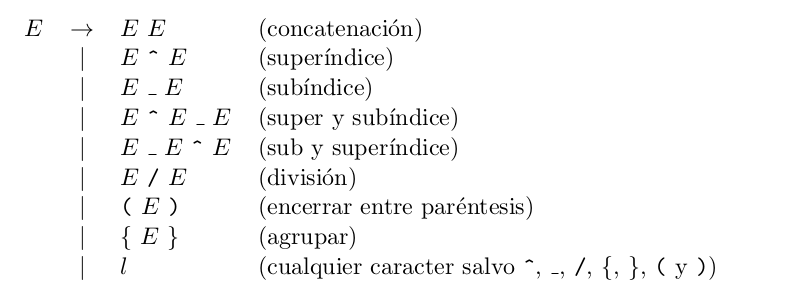
\includegraphics[width=0.9\textwidth, height=0.22\textheight, keepaspectratio]{gramoriginal}
    \caption{Gramática original a parsear según enunciado.}
    \label{fig:gram_original}
\end{figure}

Como \emph{PLY}, la herramienta que usamos tanto para el análisis lexicográfico (lexer) como para parsear, usa técnicas de tablas LALR, tuvimos que hacer algunas modificaciones sobre la gramática original para poder generar una tabla de dichas características. \newline

Una de ellas fue juntar las producciones \emph{"superíndice"} y \emph{"super y subíndice"} en una única usando un no-terminal nuevo $SUBEXP$ que pudiera ser anulable o generar el subíndice e idem para las producciones \emph{"subíndice"} y \emph{"sub y superíndice"}. De lo contrario una cadena con super y subíndices  como $A\super B\sub C$ podría ser generada produciendo primero un superíndice y luego un subíndice usando dos producciones tanto como usando una única producción. \newline

Otra manera de sortear este problema hubiera sido eliminando las producciones que combinan super y subíndices y usando ambas producciones de manera consecutiva, pero preferimos mantener las producciones ternarias sobre las binarias para facilitar el recorrido y "decorado" de la estructura sintáctica (sino no se nos complicaría distinguir estructuras de cadenas como $ A\sub \{B\super C\} $ ó $\{A\sub B\}\super C$ de las de $A\sub B\super C$). \newline

El otro cambio importante fue agregar otro no-terminal $UNARYEXP$ que genera producciones 'unarias' (paréntesis o llaves sobre una $E$, o un $CHR$). La idea viene de la necesidad de desambiguar expresiones como $E\super E\sub E$ que podrían ser generadas como $E \Rightarrow E \super  E\ SUBEXP \Rightarrow E\super E\sub E$ o como $E \Rightarrow  E \super  E\ SUBEXP \Rightarrow E \super  E \Rightarrow E\ \super  E\sub \ E\ SUPEREXP \Rightarrow E \super  E\sub \ E\ $. \newline

Como según el enunciado ni los '\super ' ni los '_' son asociativos y además $E\sub  E \super  E$ y $E\super  E \sub  E$ son equivalentes, viendo expresiones de la pinta $E_1 \sub  E_2 \super  E_3$ se puede ver que ninguno de los tres no-terminales pueden producir nunca otro subíndice o superíndice en el mismo 'scope' de paréntesis o llaves. Esto es porque siempre podríamos invertir el orden usando la equivalencia mencionada anteriormente de modo que se asocien dos de estos símbolos. \\
Tampoco pueden producir concatenaciones o divisiones porque '\super' y '_' tienen mayor precedencia que estos, por ejemplo la cadena $A\super BC$ (escribiendo los terminales $CHAR$ como sus valores para mayor claridad) no tiene la estructura de $A\super \{BC\}$ sino de $A\super B$ concatenado a $C$ \footnote{idem para subindexación} y en el caso de $A/B\super C\sub D$ primero se resuelve la indexación de B y luego la división por lo tanto la estructura se corresponde a $A/\{B\super C\sub D\}$ \footnote {idem si fuera concatenación}.

Con todos estos cambios aún seguimos teniendo problemas de tipo \emph{Shift/Reduce} y \emph{Reduce/Reduce} en nuestras tablas, que resolvimos declarando las siguientes precedencias:

Tabla de precedencia (en orden creciente)
\begin{itemize}
	\item \textbf{DIV} asociativa a izquierda

    \item '\{', '(' asociativas a izquierda
    \item \textbf{CHR} asociativa a izquierda
    \item CONCAT, asociativa a izquierda, pseudosímbolo para la concatenación
    \item \verb|'^'| no asociativa
    \item \verb|'_'| no asociativa
\end{itemize}

Las reglas de la concatenación, división e indexación siguen la descripción del enunciado mientras que las que se corresponden a $Primeros(E)$ sirven para resolver en favor de \emph{Shifts} cuando se llega al final de la expresión de una división y se está por ver una concatenación (es decir, \textbf{DIV} tiene menos precedencia que los 'primeros' de $E$ y que las otras operaciones) y que se tome \emph{Reduce} cada vez que se vió una concatenación si se está por ver una expresión concatenada o de división \footnote{Esto en teoría alcanzaría con declarar a CONCAT como asociativa a izquierda y de mayor precedencia que la división, pero al parecer para que \emph{Yacc} pueda resolver conflictos comparando orden de precedencias de símbolos con órdenes de precedencias de producciones hace falta cierta completitud sobre las declaraciones de precedencia de los símbolos que puedan llegar a ser el token corriente al decidir si reducir o no usando una producción.}.

\subsection{AST}

Como \emph{Yacc} solo nos permite sintetizar atributos únicamente en una \quotes{pasada} sobre el árbol de parsing y como veremos en la sección de atributos requerimos requerimos de varias pasadas para setear los atributos deseados, decidimos sintetizar como atributo de la gramática justamente su \emph{AST} para luego poder recorrerlo múltiples veces decorándolo. \newline

La idea es sencilla: por cada producción de la gramática sintetizamos un nodo que simboliza una operación sobre sus subtérminos. Por ejemplo, el input \texttt{A/B+C\super D\sub E} se corresponde con la estructura: \newline \texttt{DivExpr(Chr(A),Concat(Concat(Chr(B),Chr(+)),SuperSub(Chr(C), Chr(D), SubSuffix(Chr(E)))))} \newline

Cabe mencionar que no asignamos nodos a producciones de tipo '\texttt{E $\rightarrow$ UNARYEXP}' dado que no aportan nada en cuanto a términos sintácticos. Lo mismo para las llaves que solamente sirven para indicar precedencias a la hora de parsear las cadenas.

\subsection{Atributos y SVG}

Para poder generar un SVG partiendo del AST ya sintetizado, necesitamos decorarlo con atributos:

\begin{itemize}
	\item \textbf{e}: el interlineado o escala \emph{(heredado)}
	\item \textbf{a}: ancho de una expresión \emph{(sintetizado)}
	\item \textbf{h1}: corrimiento \quotes{para arriba} desde la base de una expresión \emph{(sintetizado)}
	\item \textbf{h2}: corrimiento \quotes{para abajo} desde la basa de una expresión \emph{(sintetizado)}
	\item \textbf{h}: cuánto abarca la expresión de largo la expresión en total \emph{(sintetizado)}
	\item \textbf{x}: ubicación en el eje x de una expresión \emph{(heredado)}
	\item \textbf{y}: ubicación en el eje y (la esquina \texttt{(0,0)} se corresponde con la esquina superior izquierda del buffer) de una expresión \emph{(heredado)}
	\item \textbf{svg}: output en términos de tags SVG generados por la expresión \emph{(sintetizado)}
\end{itemize}

La manera de hacer pasadas sobre el AST se corresponde a la metodología del patrón de diseño \emph{\quote{Visitors}} comunmente usado para iterar este tipo de estructuras y que permite usar polimorfismo y double-dispatch para hacer llamados recursivos sobre cada nodo.

\subsubsection{Cálculo de atributos}
A continuación explicamos coloquialmente cómo fuimos generando los atributos para decorar el AST.

\begin{itemize}
	\item El atributo \textbf{\quotes{e}} correspondiente a la escala, se inicia en 1 sobre la raíz y se reduce a un 70\% de su valor en cada indexación. Se trata de un atributo heredado.

	\item El atributo \textbf{\quotes{a}} correspondiente al ancho es:
	\begin{itemize}
		\item el 60\% de la escala para caracteres
		\item suma de anchos de subexpresiones el caso de concatenaciones
		\item suma del ancho de la expresión principal y máximo ancho entre los índices para indexaciones
		\item máximo entre ancho del numerador y del denominador para divisiones
		\item suma de la expresión mas ancho de los dos paréntesis para dicho caso
	\end{itemize}

	\item El atributo \textbf{\quotes{h1}} lo sintetizamos con los siguientes valores:
	\begin{itemize}
		\item el interlineado para caracteres
		\item máximo entre ambos $h1$ para concatenaciones
		\item máximo entre el $h1$ de la expresión principal y $h1$ del superíndice mas su altura desde la base de la expresión general
		\item $h1$ del numerador menos el corrimiento para arriba desde la base de la línea de división para tales expresiones
		\item $h1$ de la expresión principal para paréntesis
	\end{itemize}

	\item El atributo \textbf{\quotes{h2}} es:
	\begin{itemize}
		\item 0 para caracteres
		\item máximo entre ambos $h2$ para concatenaciones
		\item máximo entre $h2$ de la expresión principal y el $h2$ del subíndice mas su desfasaje con la base de la expresión principal considerando tambien que las letras miden el 70\% del interlineado desde el $y$ hasta su base real. \footnote{La idea de considerar el corrimiento real desde la base del caracter y no del interlineado es que no se produzcan paddings fantasma en las divisiones (que corresponderían al espacio que queda entre la base del caracter y de su interlineado). Para paréntesis por ejemplo es 80\%. Se podría ir ajustando el porcentaje de acuerdo a cada caracter, pero como nos pareció que el padding generado por esta diferencia era casi despreciable además de que se espera que las expresiones sean principalmente letras y caracteres aritméticos decidimos estandarizar el porcentaje de las letras.}
		\item $h2$ del denominador mas el corrimiento para arriba desde la base de la línea de división para las divisiones
		\item $h2$ de la expresión principal para paréntesis
	\end{itemize}

	\item El atributo \textbf{\quotes{h}} se calcula como:
	\begin{itemize}
		\item $h1$ para caracteres
		\item $h$ de la expresión principal para paréntesis
		\item suma de $h1$ y $h2$ para las demás operaciones
	\end{itemize}

	\item El atributo \textbf{\quotes{x}} se inicializa en 0 en la raíz y lo heredamos en cada caso como:
	\begin{itemize}
		\item el mismo $x$ pasado como parámetro para caracteres
		\item el mismo $x$ pasado como parámetro para la primer expresión de una concatenación y el $x$ parámetro sumado al ancho de la primer expresión para la segunda
		\item el mismo $x$ pasado por parametro más la mitad de la diferencia entre el máximo de los dos anchos y el ancho del numerador o denominador según el caso, de modo que ambas expresiones queden verticalmente centradas
		\item el mismo $x$ argumento para las expresiones principales y ese mismo x mas el ancho de la expresión principal para los índices en las indexaciones
		\item $x$ argumento mas el ancho de un paréntesis para la expresión principal para los paréntesis
	\end{itemize}

	\item El atributo \textbf{\quotes{y}} tambien se inicializa en 0 en la raíz y lo heredamos como:
	\begin{itemize}
		\item el mismo $y$ subido $h2$ del numerador para él mismo y bajado $h1$ del denominador para este, ambos casos con un desplazamiento hacia arriba por el corrimiento de la barra de división
		\item el mismo $y$ argumento bajado un cuarto del $h$ de la expresión total para subíndices mientras que nuevamente el mismo $y$ subido $0.45$ veces el h1 de la expresión principal para superíndices
		\item para los paréntesis, caracteres y concatenación se mantiene igual la altura
	\end{itemize}

	\item El atributo \textbf{\quotes{svg}} se toma concatenando los strings de las subexpresiones:
	\begin{itemize}
		\item para caracteres se devuelve un tag de tipo text con 'x', 'y' y 'font-size' correspondientes a los atributos $x$, $y$ y $e$ del mismo
		\item para divisiones se concatenan los SVG del numerador y denominador con una barra horizontal de longitud del ancho de la división a casi la mitad del interlineado de altura
		\item para paréntesis se concatenan tags de texto con caracteres '(' y ')' escalados para ocupar el 'h' de la expresión \footnote{Como dijimos antes, los paréntesis ocupan un 80\% de longitud del interlineado por lo que hay un 20\% de espacio vacío que, al escalarse, tambien se multiplica por lo que se lo restamos de modo que solamente quede un 20\% del interlineado como tal espacio.}
	\end{itemize}
\end{itemize}

\clearpage

\clearpage

\end{document}

